\chapter{Robotic VLMs}

\section{Robotic Foundation Models}
\subsection{What is a Robotic Foundation Model?}
No explicit representation of states / transition functions. We need a policy that maps (observaition/state, goal) to some action. With current foundational vision-and-language models, the output may not always be perfect,
but it will always generate something reasonable. \\ 

\noindent \textit{The synthesized action may not always be optimal, but the generated trajectory will 
always be beautiful and reasonable.}

\subsection{Existing Works}
Current works are parameter-wise heavy ($\sim$55B parameters), closed source, and lack fine tuning.

\section{OpenVLA I}
This model consists of 7B parameters, fully open-source, and supports efficient fine-tuning. OpenVLA I outperformed SOTA RT-2-X (55B) by 16.5\% in absolute task success rate. It 
demonstrated effectiveness of modern parameter-efficient fine-tuning and quantization. This was the first open-source 
generalist VLA, thus supports future research.

\subsection{Architecture}

\begin{figure}[hbpt!]
  \centering
  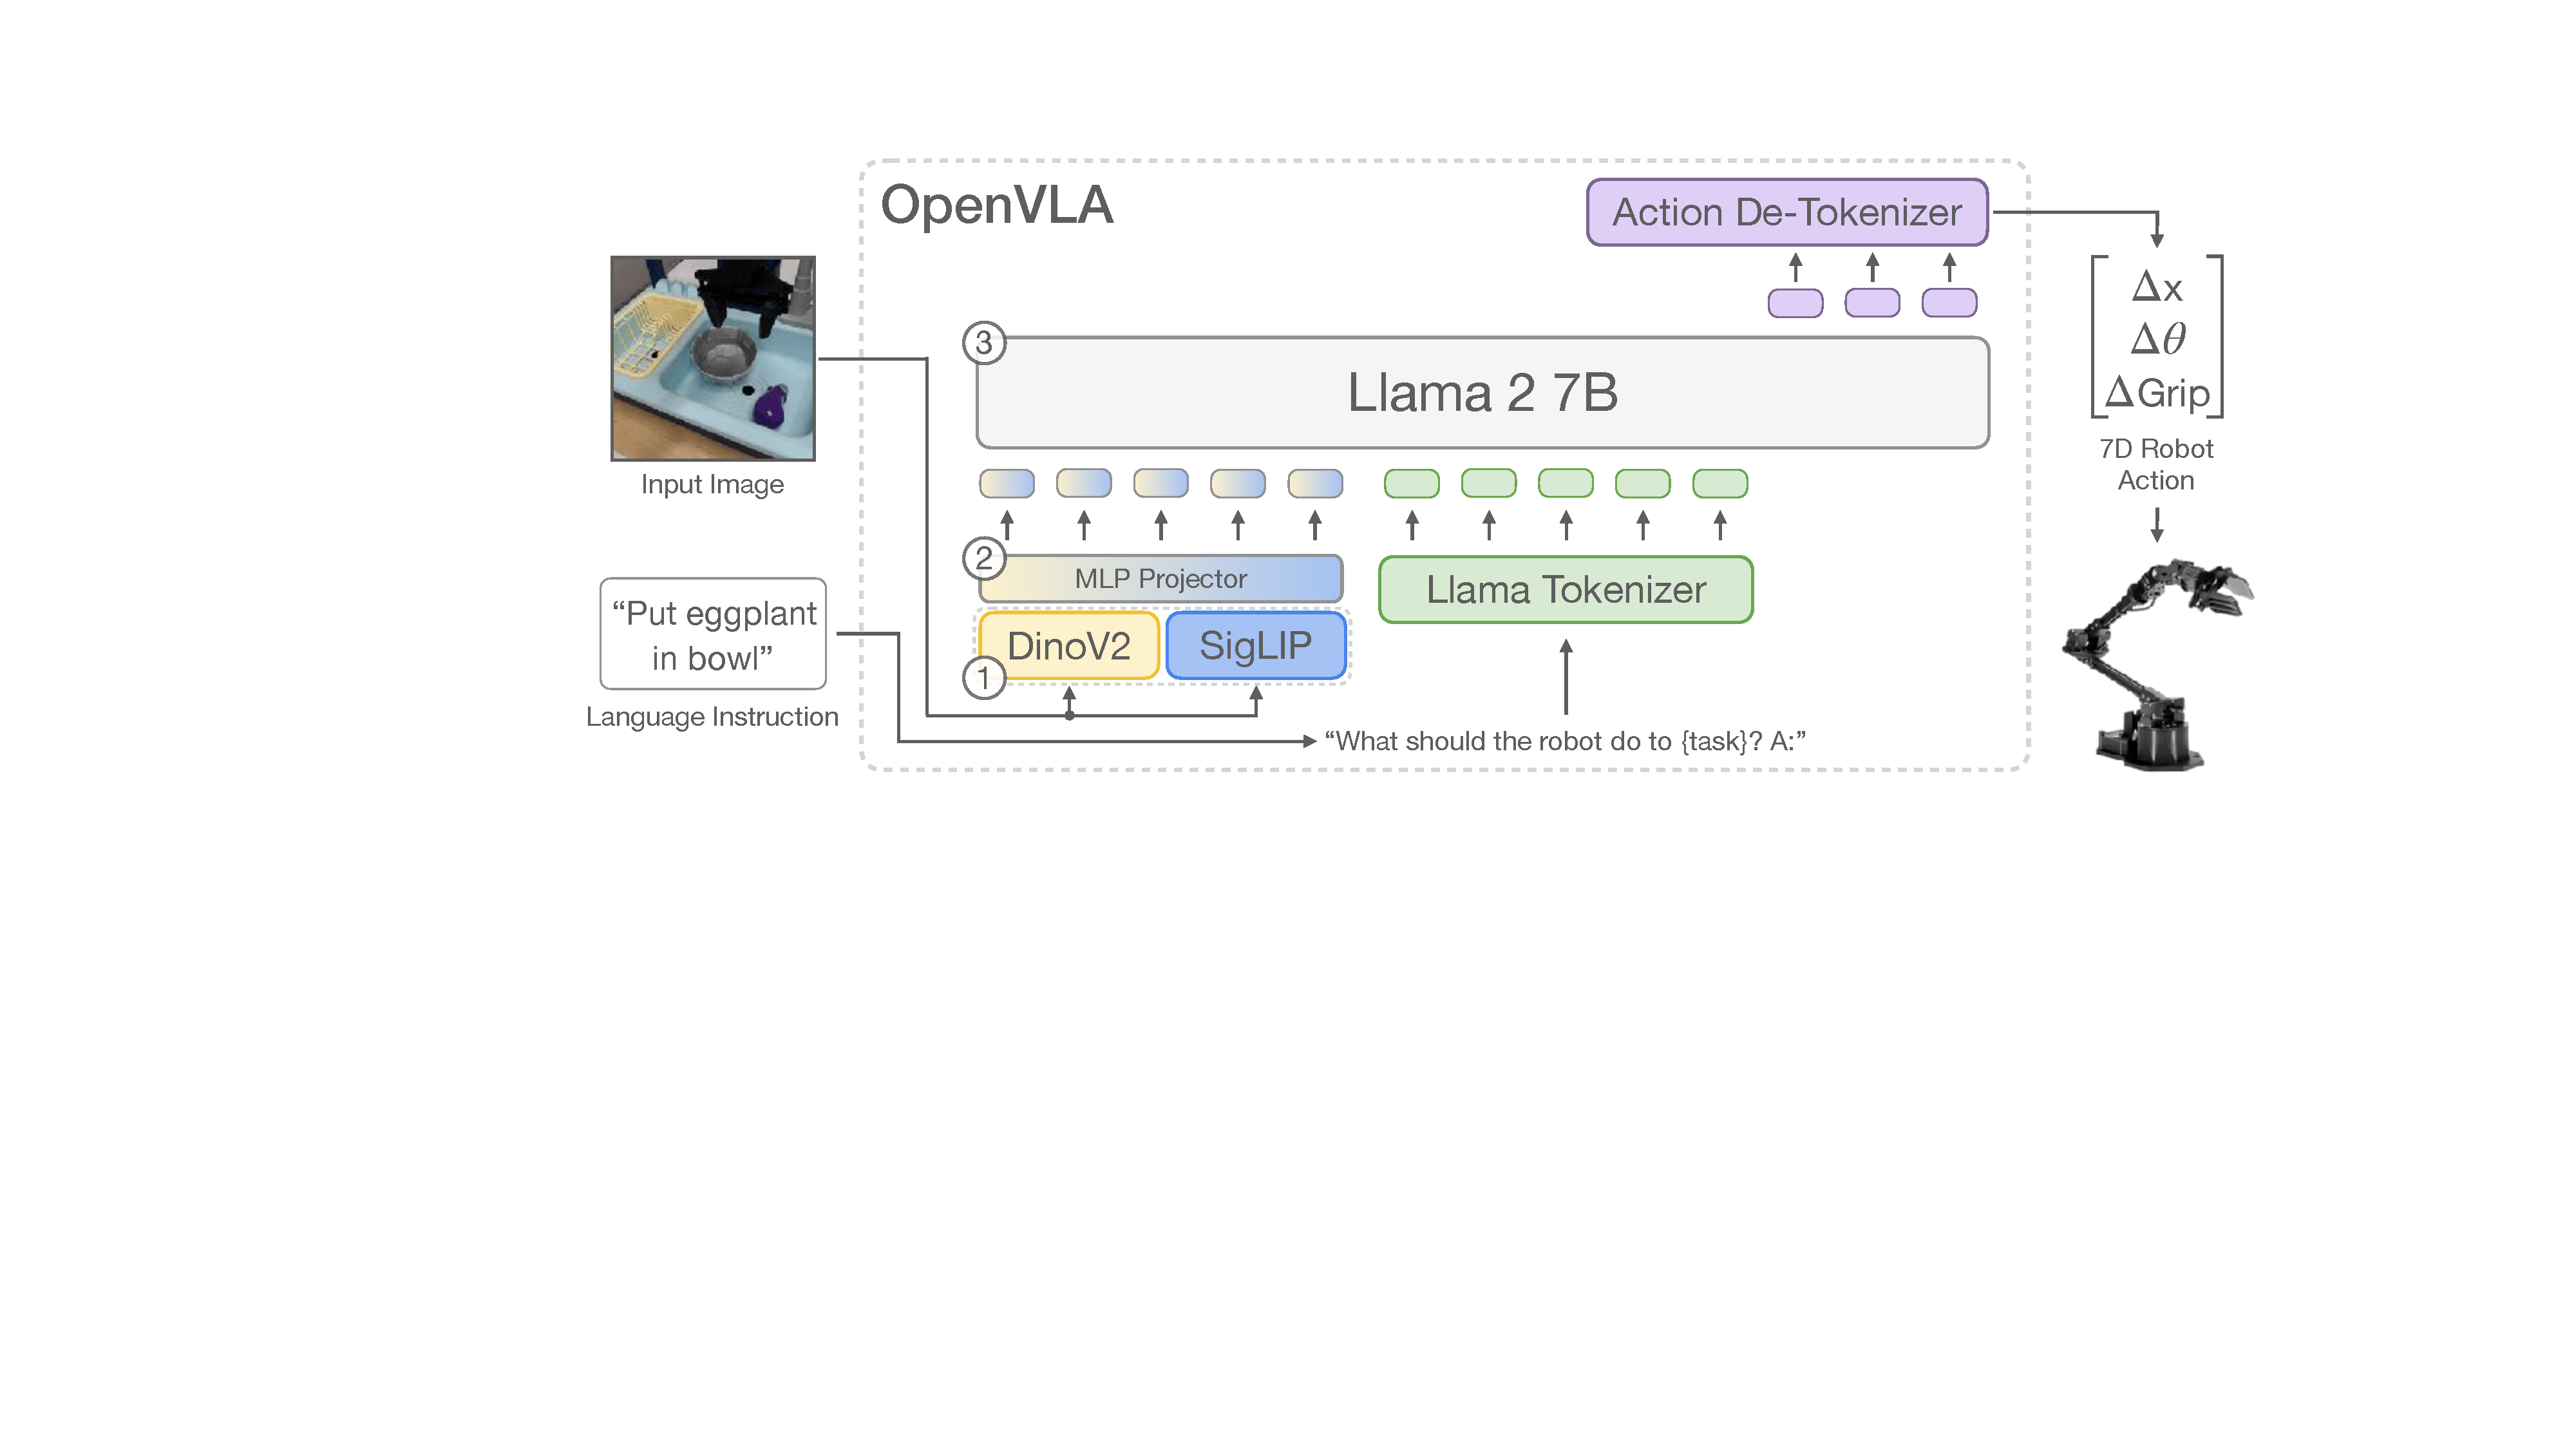
\includegraphics[width=0.75\textwidth]{chapters/openvla_model.pdf}
  \caption{OpenVLA architecture}
\end{figure}
\noindent OpenVLA architecture consists of three key components:
\begin{enumerate}[label=(\arabic*), topsep=5pt, itemsep=1pt]
  \item Vision encoder that concatenates Dino V2 and SigLIP features 
  \item Projector that maps visual features to the langauge embedding space 
  \item Llama 2 7B-parameter large language model
\end{enumerate}
The model outputs a 7-dimension token: $[$$\Delta$x, $\Delta$y, $\Delta$z, $\Delta$roll, $\Delta$pitch, $\Delta$yaw, gripper status$]$.

\subsection{Training}
Training data is the open X-Embodiment dataset 70 robot dataset with 2M trajectories. Curated under 
below conditions, selected 970k robot episodes:
\begin{enumerate}[label=(\arabic*), topsep=5pt, itemsep=1pt]
  \item Single arm manipulations, with 3rd person view camera 
  \item Ensure a balanced mix of embodiments, task, scenes
\end{enumerate}
OpenVLA model is trained on a cluster of 64 A100 GPUs for 14 days. Inference: 15GB of GPU memory when loaded bfloat16.

\subsection{Generalization}
Settings: robot and tasks from pre-trained data. WindowX robot from BridgeData V2 evaluation. Mobile manipulation robot from RT-1 and RT-2 evaluation. \\ 

\noindent Categorizing the term "Generalization":
\begin{enumerate}[label=, topsep=5pt, itemsep=0pt]
  \item \textbf{Visual}: unseen backgrounds, distractor objects, appearances of objects 
  \item \textbf{Motion}: unseen object positions/orientations 
  \item \textbf{Physical}: unseen objects sizes/shapes 
  \item \textbf{Semantic}: unseen target objects, instructions, concepts from the internet
\end{enumerate}

\subsection{Efficient fine-tuning}
Adapting a pretrained VLA model to a new robot, new environment, or new task. Quick adaptation to a new setup, with a much smaller dataset. Implicitly captures per-setup differences (camera pose, embodiment, environment, reference frame, etc...). Diffusion 
policy is good for narrow, single-instruction tasks. Fine-tuned VLAs are better with multiple objects and langauge conditioning. Robot data pretraining provides significant performance boost. OpenVLA shows strong 
performance across task types.
\subsection{Parameter-efficient FT}
Tested different fine-tuning strategies (full FT, last layer only, frozen vision, sandwich, LoRA). The critera for this was memory requirement and performance. Authors found LoRA is efficient, with minimal 
performance degradation. \\ 

\noindent \textbf{LoRA}: low-rank adaptation of large language models.
\begin{enumerate}[label=(\alph*), topsep=5pt, itemsep=0pt]
  \item Vanilla fine-tuning: update $(d \times h)$ weights, very expensive
  \item LoRA: only train $B$ and $A$, where $BA = \Delta W$ (weight updates)
  \item Insight: pretrained $W$ is near a good solution; for fine-tuning updating all weights is unnecessary
\end{enumerate}

\subsection{Quantization}
Many foundation models require large GPU memory (even for inference). Idea: reduce the precision 
(\# of bits used) of model weights $\rightarrow$ less memory footprint, extra quantization / dequantization overhead, increased arithmetic error. Here there is a 
memory-performance tradeoff.

\subsection{Summary}
Open-source VLA model for manipulators (image + language instruction $\rightarrow$ robot action). CV \& NLP advancements on robotic applications. Towards
large, 'generalist', widely-deployable robot models: robot data pretraining $\rightarrow$ general performance; fine-tuning (LoRA) $\rightarrow$ task-specific adaptation; quantization $\rightarrow$ memory-efficient inference.

\section{Pi-Zero (Physical Intelligence)}

\begin{figure}[hbpt!]
  \centering
  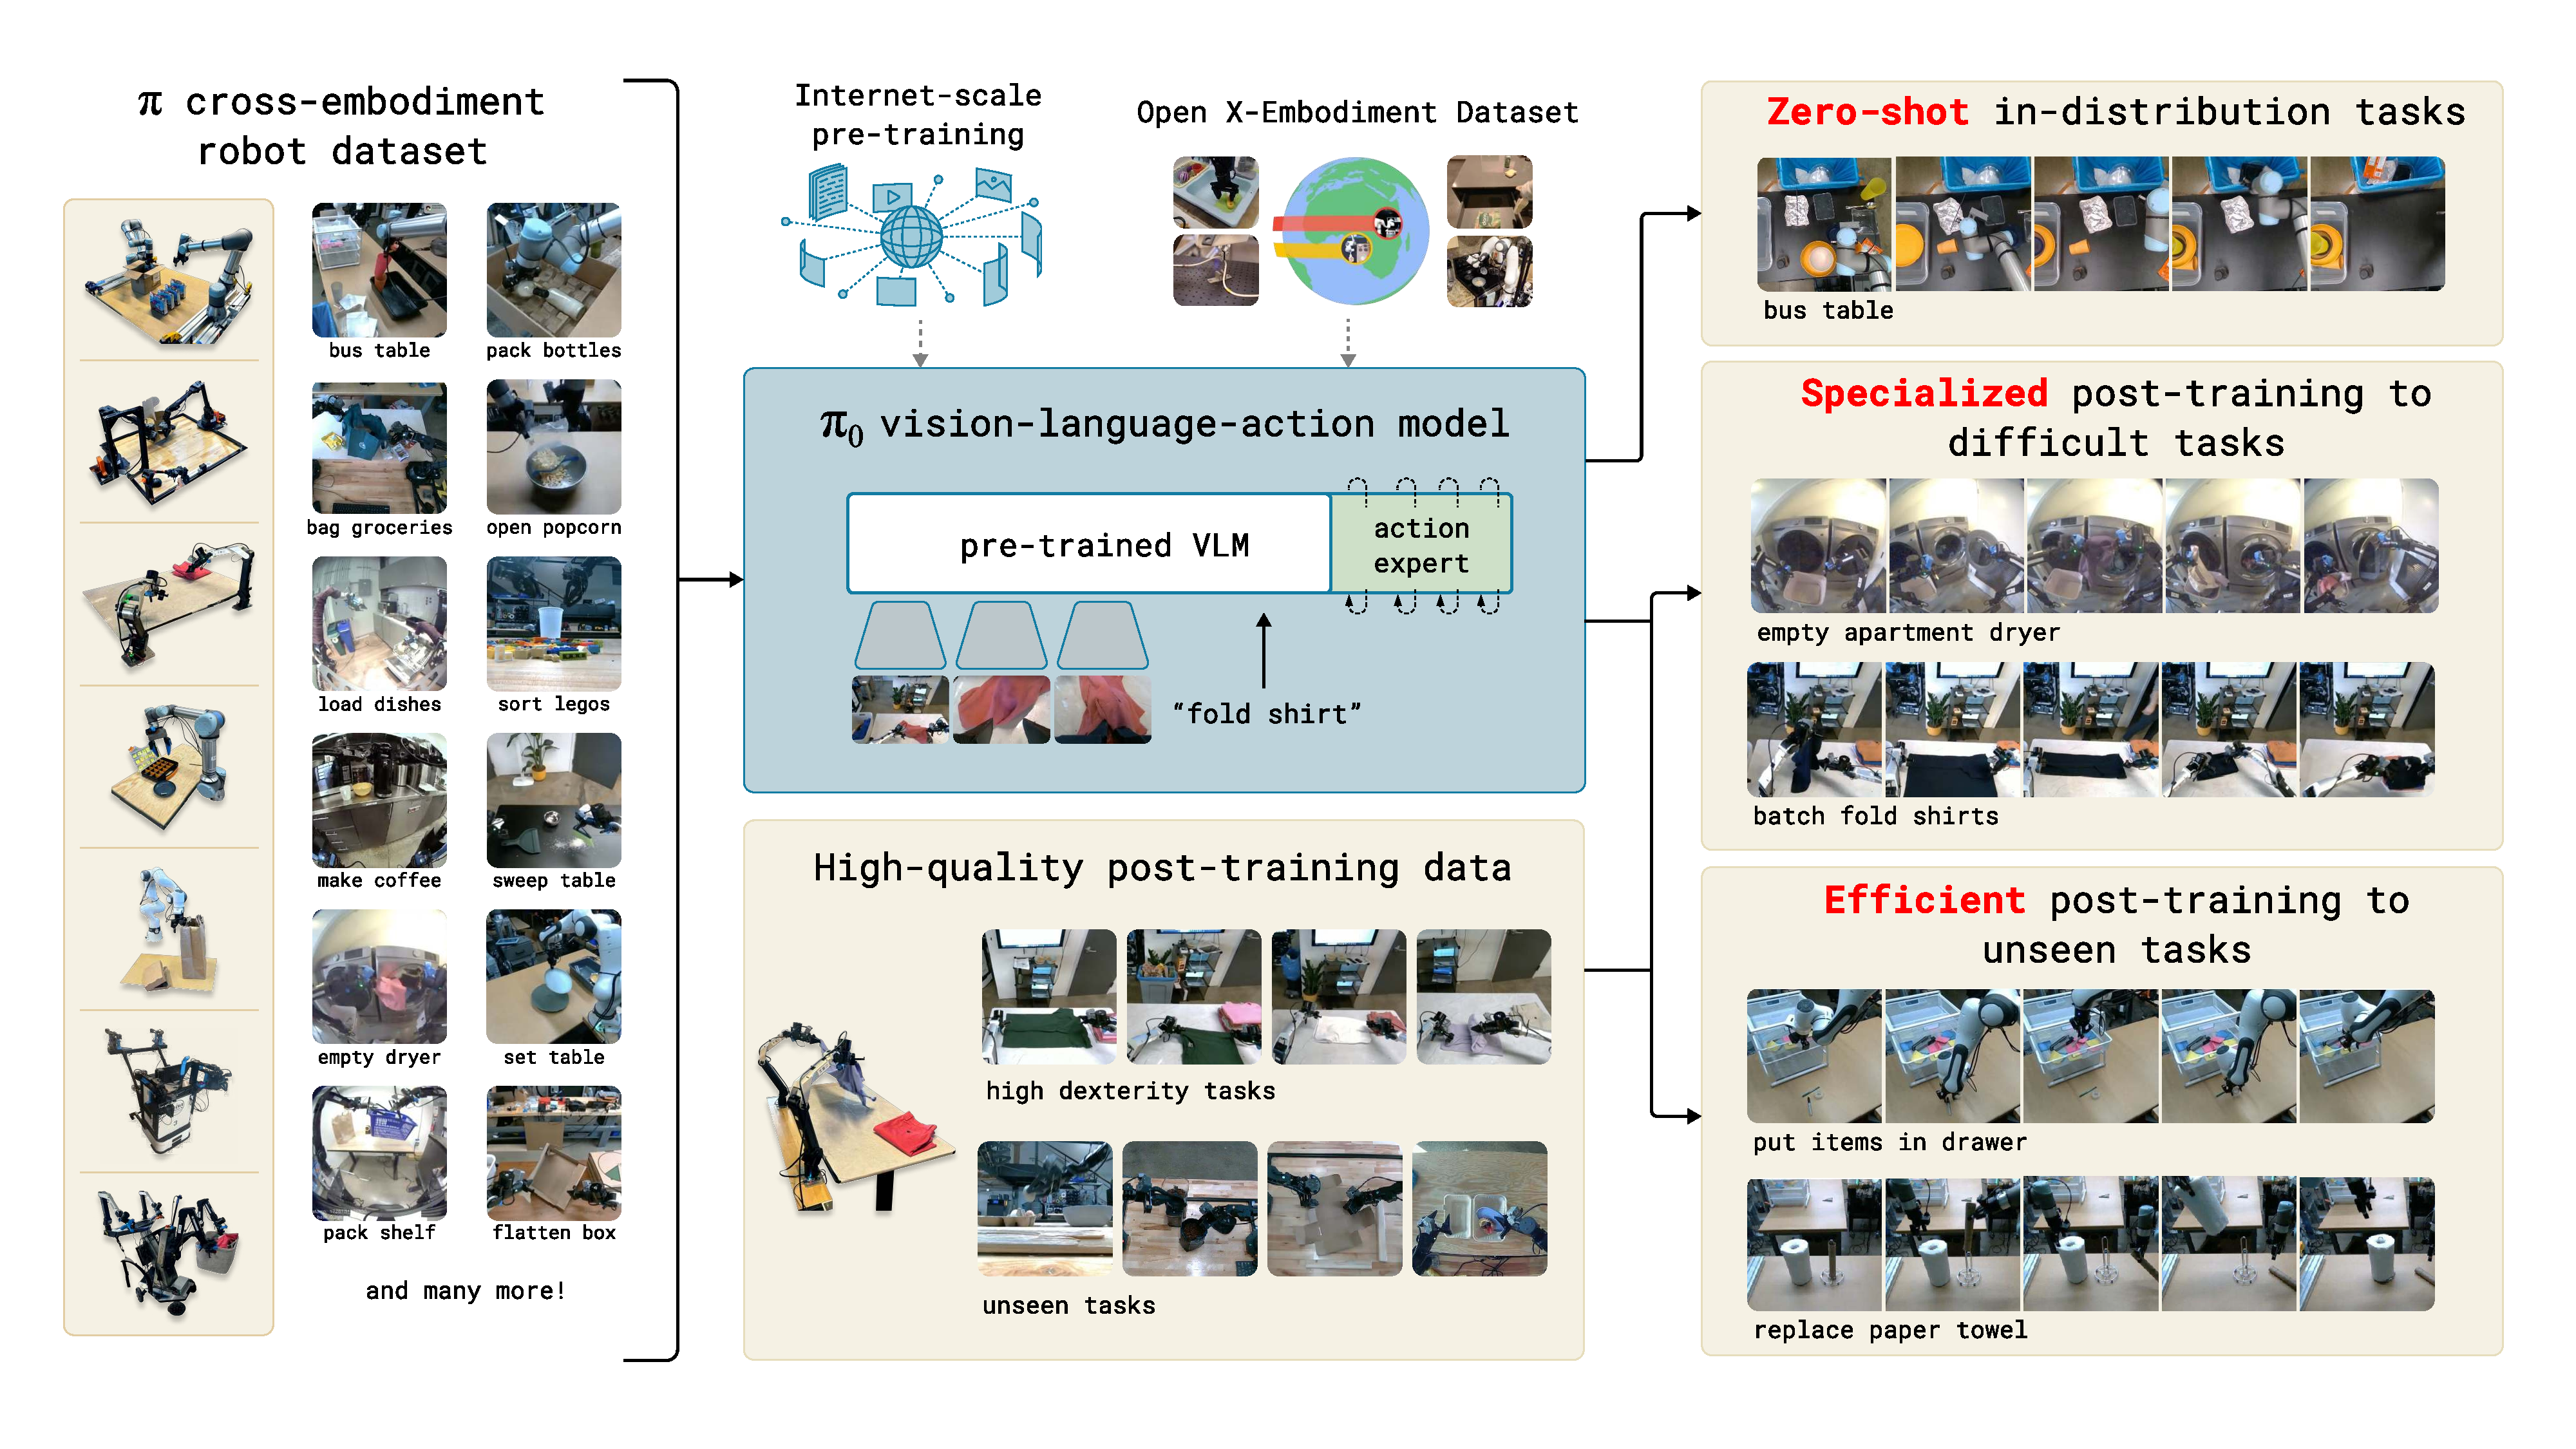
\includegraphics[width=\textwidth]{figures/teaser_fig_compressed.pdf}
  \vspace*{-1.25cm}
  \caption{$\pi_0$ model}
\end{figure}

\begin{figure}[hbpt!]
  \centering
  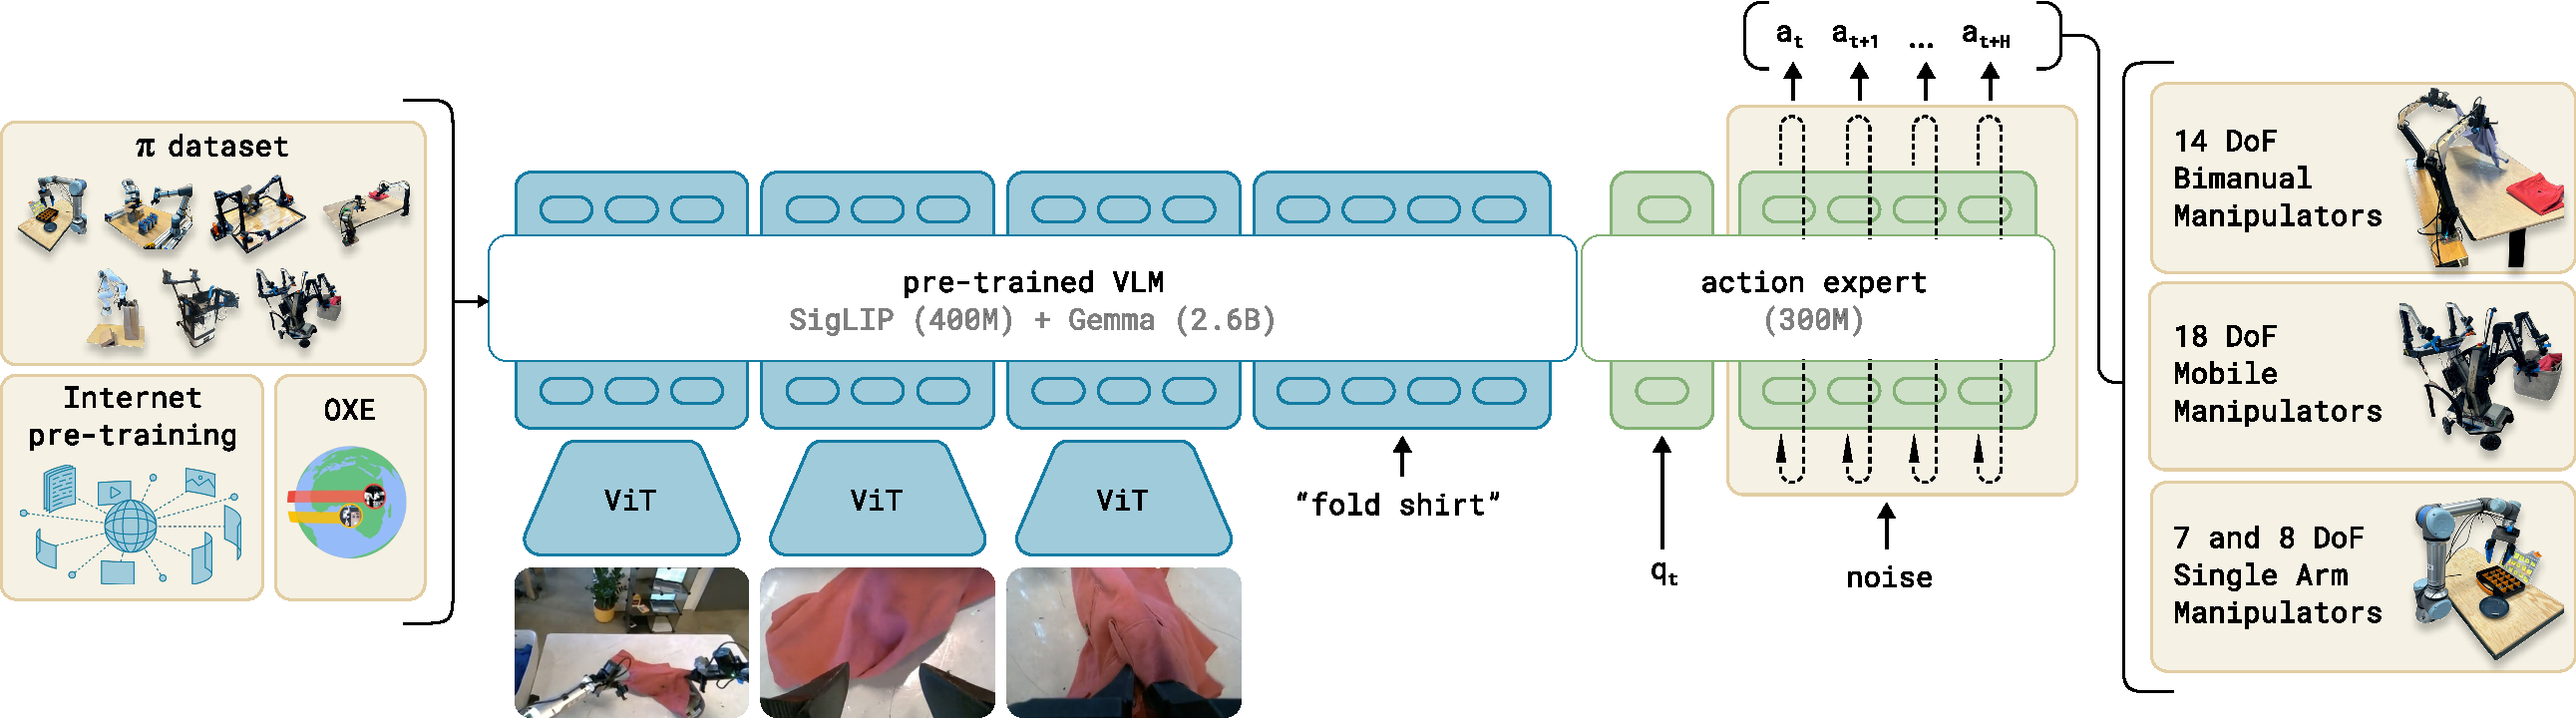
\includegraphics[width=\textwidth]{figures/overview.pdf}
  \vspace*{-0.75cm}
  \caption{$\pi_0$ overview}
\end{figure}

\subsection{Performance vs OpenVLA}
The full pre-trained $\pi_0$ model performs...
